% Template for ICASSP-2010 paper; to be used with:
%          spconf.sty  - ICASSP/ICIP LaTeX style file, and
%          IEEEbib.bst - IEEE bibliography style file.
% --------------------------------------------------------------------------
\documentclass{article}
\usepackage{spconf,amsmath,graphicx}
\usepackage{url}
\usepackage{verbatim}

% Example definitions.
% --------------------
\def\x{{\mathbf x}}
\def\L{{\cal L}}

% Title.
% ------
\title{IMPUTATION OF BEAT-ALIGNED FEATURES AND MUSIC PATTERN LEARNING}
%
% Single address.
% ---------------
%\name{Thierry Bertin-Mahieux\thanks{Thanks to NSERC and some other stuff.}}
%\address{EE dept., Columbia University}
%
% For example:
% ------------
%\address{School\\
%	Department\\
%	Address}
%
% Two addresses (uncomment and modify for two-address case).
% ----------------------------------------------------------
\twoauthors {Thierry Bertin-Mahieux\sthanks{TBM is supported in part
    by a NSERC PG scholarship.}, Graham Grindlay,} {Columbia
  University\\ LabROSA\\ New York, USA} 
   {Ron J. Weiss\sthanks{supported by NSF grant IIS-0844654 and Institute of
    Museum and Library Services grant LG-06-08-0073-08.}  and Daniel
  P.W. Ellis\sthanks{This work was supported in part by the NSF grant
    IIS-0713334.  Any opinions, findings and conclusions or
    recommendations expressed in this material are those of the
    authors and do not necessarily reflect the views of the sponsors.}} 
{New York University / Columbia University\\ MARL / LabROSA\\ New
  York, USA}

\begin{document}
\ninept
%
\maketitle
%
\begin{abstract}
Imputation is cool. It is a well-defined problem, as opposed to segmentation.
Gives a reasonable benchmark to compare algorithms that claim learning meaningful
patterns on music. Hard to beat benchmarks comparison, for instance linear
prediction. We compare some methods and discuss contradicting error measures. 
We'll track you down if you don't accept this paper.
\end{abstract}
%
\begin{keywords}
Missing data, chroma features, beat imputation, codebook learning
\end{keywords}
%
\section{Introduction}
\label{sec:intro}
Many signals show similarities and repetitions over time.  
%Learning these repetitions in an unsupervised way remains a challenge. 
Finding robust patterns may prove useful for tasks such as song
similarity (recognizing songs with similar patterns), song
segmentation (labeling chorus/verse structure), and cover song
recognition (identifying songs with similar high-level patterns).
Therefore, we are looking for patterns that not only explain the
low-level signal, but also contain musical characteristics.  However,
it is unclear how to evaluate the quality of these patterns.  In this
paper, we propose a task based on missing data imputation and discuss
various performance metrics which are sensitive to musically
meaningful aspects of the data.  

Imputation refers to a family of techniques used to fill in missing
data entries.  Previous work on audio-related applications has
included speech denoising~\cite{Raj1998}, speech
enhancement~\cite{Sanneck1996}, and model
evaluation~\cite{Smaragdis2009,Hoffman2010}.  However, to the best of
our knowledge, previous research has only considered a few missing
time-frequency \emph{bins}.  In contrast, we define an imputation task
where there are many consecutive time frames missing.  We refer to
this task as \emph{multi-frame} imputation.  This makes the problem
more challenging, but also allows us to more carefully evaluate the
temporal aspects of our model.  % needs to be reworded?
% mention real-world packet-loss case?

\begin{comment}
and fully masking consecutive beats of music have not been
considered. A real-life analogous problem would be a music stream
signal that is lost for a few seconds. The goal here would be to infer
a reasonable stream to replace the original one. Thus we do not only
want a signal close to the original in a reconstruction sense, but
also a signal that has similar ``musical properties'' to the user
ear. These properties are difficult to define, but we refer to higher
order dependencies present in the signal. For instance, the rate of
note onsets, the number of notes activated at the same time, and other
texture-like elements. We will argue that entropy is a good
approximation of these characteristics.
\end{comment}

Figure \ref{fig:types} shows three matrices with different amounts of
missing data.  As mentioned previously, other researchers
\cite{Smaragdis2009} have worked with the partially missing data (see
Figure~\ref{fig:types}).  A slightly more complex problem can be
defined by masking out an entire time frame.  This problem is
illustrated in Figure~\ref{fig:types}.  It is worth noting that due to
our data representation (see Section~\ref{ssec:feats}), the
single-frame imputation problem is somewhat easy.  In contrast, the
problem of multiple missing frames (see Figure~\ref{fig:types}) can be
made arbitrarily difficult.

\begin{comment}
a few frequency bins are hidden and can be
recovered from their neighborhood, both in time and frequency. Masking
one full beat is a natural extension, and the solution is easy as
music notes are often sustained over many beats. Two or three missing
beats remain solvable as music bare many repetitions. One can usually
find a similar section from an unmasked part of the song (think about
a repeated chorus for instance).  The real challenge arises from
masking many consecutive beats.
\end{comment}

Music highly structured in time and as such is particularly suitable
for the imputation task.  In addition to musicological implications,
large-scale models of music data have numerous commercial
applications, including recommendation systems, digital rights
management, and creative tools.  

Figure \ref{fig:basic} shows an example of multi-frame imputation of
music data.  Linear regression, which explicitly minimizes Euclidean
distance, is used to impute the missing data in
Figure~\ref{fig:basic}.  However, it is clear from visual inspection
that linear regression yields an overly-smooth reconstruction.  In
fact, we argue that a more extensive set of metrics is needed for
proper evaluation.


\section{TASK DEFINITION}
\label{sec:task}

\subsection{DATA AND FEATURES}
\label{ssec:feats}
We represent music using chroma features \cite{Ellis2007a}. They
record the intensity associated with each of the 12 semitones
(e.g. piano keys) within one octave, but all octaves are folded
together. One can see them as a very coarse and noisy music
transcription. We use an online API \cite{EchoNest} that implements
chromas over a constant-Q spectrogram.  Also, music has a natural time
metric expressed in beats. Therefore, missing frames are equivalent to
missing all features for the length of one beat. Accordingly, we
resample the features so that each chroma vector spans one beat. Note
that music beat tracking algorithms perform relatively well
\cite{Davies2007} even if the task is not considered solved.

Beat-aligned chroma features have been used for cover song recognition
\cite{Ellis2007a} and segmentation \cite{Weiss2010}. In our previous work
\cite{Bertin-Mahieux2010a}, we attempt to learn music patterns in that
representation. Results on multi-beat imputation are done on a random
subset of $5K$ songs of the cowbell dataset
\cite{Bertin-Mahieux2010a}.


\begin{figure}[t]
\begin{center}
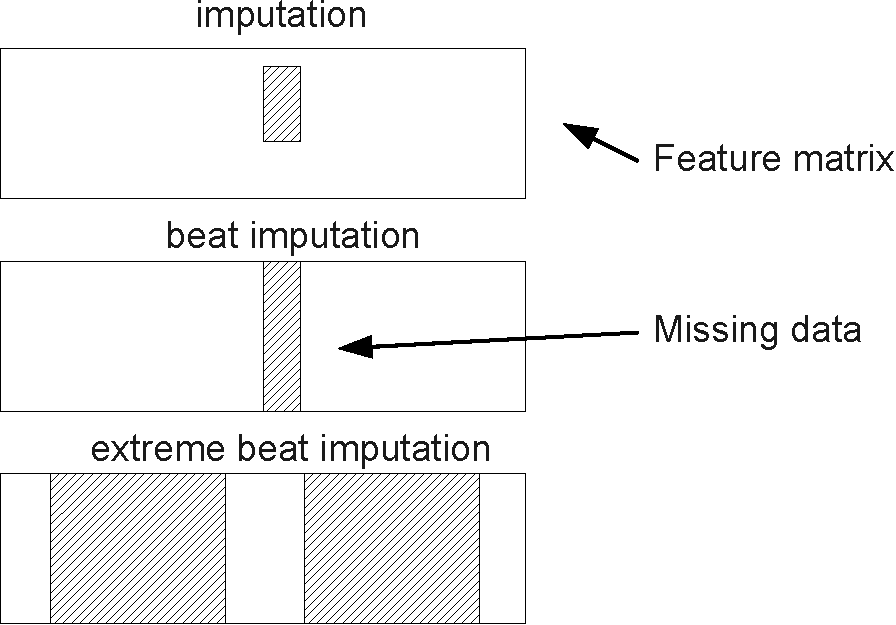
\includegraphics[width=.7\columnwidth]{type_imputation}
\end{center}
\caption{Imputation types.
\label{fig:types}}
\end{figure}

\begin{figure}[t]
\begin{center}
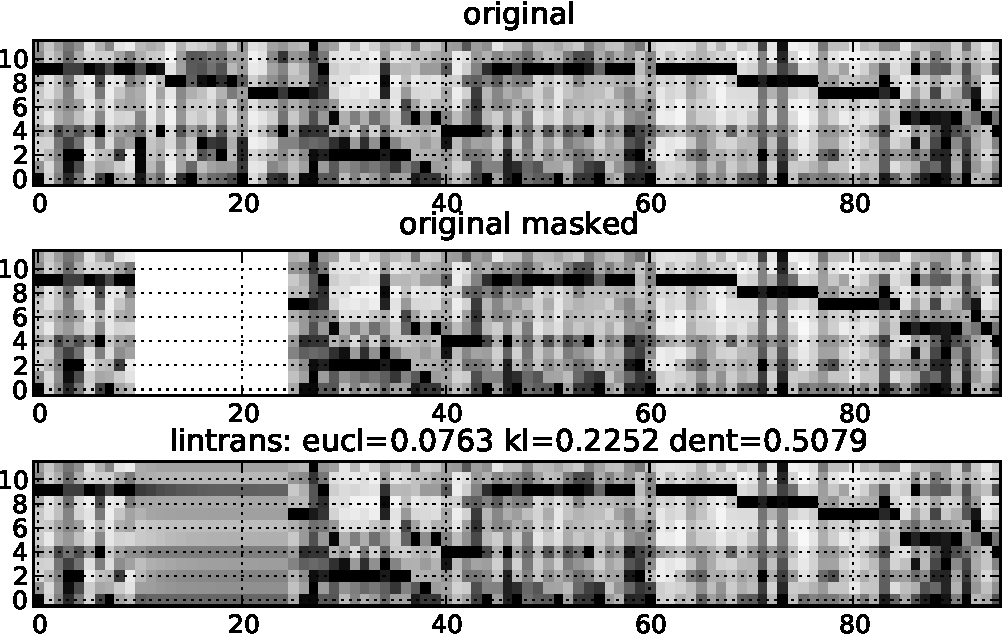
\includegraphics[width=.95\columnwidth]{basic}
\end{center}
\caption{$15$ beats imputation example, rows are 1) original 2) original masked
3) reconstruction using a linear transform of one previous beat.
\label{fig:basic}}
\end{figure}

% IPYTHON COMMAND TO RECREATE ABOVE FIGURE
%btchroma2 = sio.loadmat('/home/thierry/Columbia/covers80/coversongs/covers32kENmats/john_lennon+Double_Fantasy+05-I_m_Losing_You.mp3.mat')['btchroma']
%p1=185;p2=p1+15;mask=np.ones(btchroma2.shape);mask[:,p1:p2]=0.
%evaluation.plot_oneexample(btchroma2,mask,p1,p2,methods=['lintrans'],methods_args=[{'win':1}],measures=('eucl','kl','dent'),plotrange=(p1-10,p2+70))


\subsection{MEASURES}
\label{ssec:measures}
Euclidean distance is a natural choice for reconstruction and encoding
tasks. However, we saw from Figure \ref{fig:basic} that it can favor
unsatisfying results for multi-beats imputation. We devote a great
part of this work to exploring metrics that measure other aspects of
the reconstruction: for instance, a metric that would reward
preserving the level of granularity of the original data in Figure
\ref{fig:basic}.

We first consider Mahalanobis distances of the form $d_p =
|x_1-x_2|^p$, especially with $p \leq 2$. Figure \ref{fig:measures}
illustrates the effect of these measures on one dimensional data.  The
greyed rectangle represents the case where a reconstruction is
considered valid if it is between some $\delta$ of the original and
wrong otherwise.  Mahalanobis distance approximate this case with an
increasingly smaller $\delta$ as $p \rightarrow 0$.

Let's consider these cases on the toy example of Figure
\ref{fig:square}.  The square wave of period $1$ could be one row of
our missing data for instance.  We approximate it by two signals: the
same square wave translated by a quarter of its period and the average
function (constant at $0.5$). The average reconstruction errors on
$[0,1]$ for the translated wave, with any $d_p$, is $0.5$.  For the
average and $d_2$, this error is $0.25$.  Hence, the average function
seems the most accurate. However, with $d_1$, the errors are both
equal to $0.5$. With $d_{1/2}$, errors are now $0.5$ and
$0.71$. Hence, if the translated square wave should be a better
approximation, Euclidean distance is misleading.

%Vasicek estimator \cite{Learned-Miller2003}.  

The phenomena above explain why reconstruction such as in Figure
\ref{fig:basic} ($3$rd row) or in Figure \ref{fig:avgnnrand} ($3$rd
row) often result from powerful algorithms. Learning an overly
smoothed solution and avoiding extreme values is rewarded by some
metrics. $d_{1/2}$ seems to be a solution from the toy example in
Figure \ref{fig:square}, but we will see in Section \ref{sec:exp} that
it is not really the case in practice. 
Similarly, Kullback-Leibler
(KL) and Jensen difference \cite{Michel1994} are two measures based on
entropy, thus should not behave necessarily in the same way as $d_p$.
Once again, it is not the case in practice. We now look into other
measures that would differ from $d_2$. 
Upon visual inspection, they
should reward granularity which is missing in Figure \ref{fig:basic}
for instance. Delta chromas are the finite difference along the time
axis of the chromas. Deltas of over-smoothed solution are closed to
$0$ whereas typical songs have more varying deltas. \textbf{ddiff}
measures the absolute difference between the sum of absolute values of
the deltas for the original data and its reconstruction.

Another idea is to look at the histogram of values and compute its
entropy. Once again, sustained solutions should measure differently
than the original.  Absolute normalize difference entropy
(\textbf{D-ENT}) \cite{Mentzelopoulos2004} between two vectors is
computed as follow: we discretize $(0,1)$ in $10$ bins and create the
normalized histogram of values.  The entropy of each of the bins
$b_{bi}$ is $e_b = - log_2 b_b$ for each of the two vectors
$i$. Finally:
\[
\mbox{D-ENT} = \left( \Sigma_b \frac{e_{b1} - e_{b2}}{e_{b1}} \right) / (\mbox{\# bins})
\]
Note that D-ENT is not symmetric. In our experiment, the first vector
is the original one.  If we look at Figure \ref{fig:avgnnrand}, the
reconstruction with the lowest D-ENT is using nearest neighbor and not
averaging as with Euclidean distance.

Note that we tried other entropy related measures,
i.e. Kullback-Leibler divergence (KL) and Jensen difference
\cite{Michel1994}. As for $d_{1/2}$, they behave in a surprisingly
similar fashion as the Euclidean distance.  We explained above why
Euclidean distance justifies disappointing reconstructions. At the
same time, we do not argue that we should ignore or replace
it. Euclidean distance measures reconstruction in a fundamental
way. We believe we need a set of measures to quantify the quality of
music patterns, Euclidean distance being one of them. In the next
section, we investigate which measures behave in a similar way, thus
helping us to decide which ones are usefull to report.

\begin{figure}[t]
\begin{center}
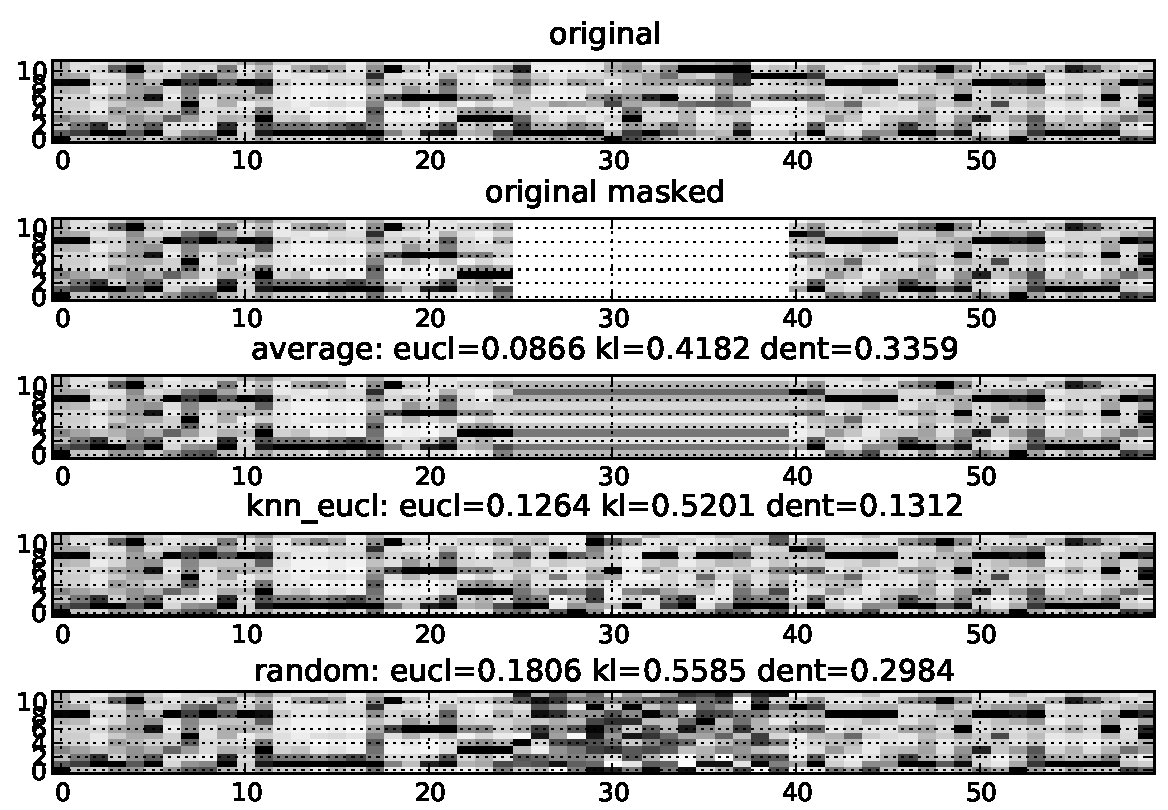
\includegraphics[width=.95\columnwidth]{avg_nn_rand}
\end{center}
\caption{Same beat imputation example as Figure \ref{fig:basic}, 
rows are 1) original 2) original masked
3) reconstruction using the average of nearby beats 4) using
nearest neighbor 5) using random.
\label{fig:avgnnrand}}
\end{figure}

\begin{figure}[t]
\begin{center}
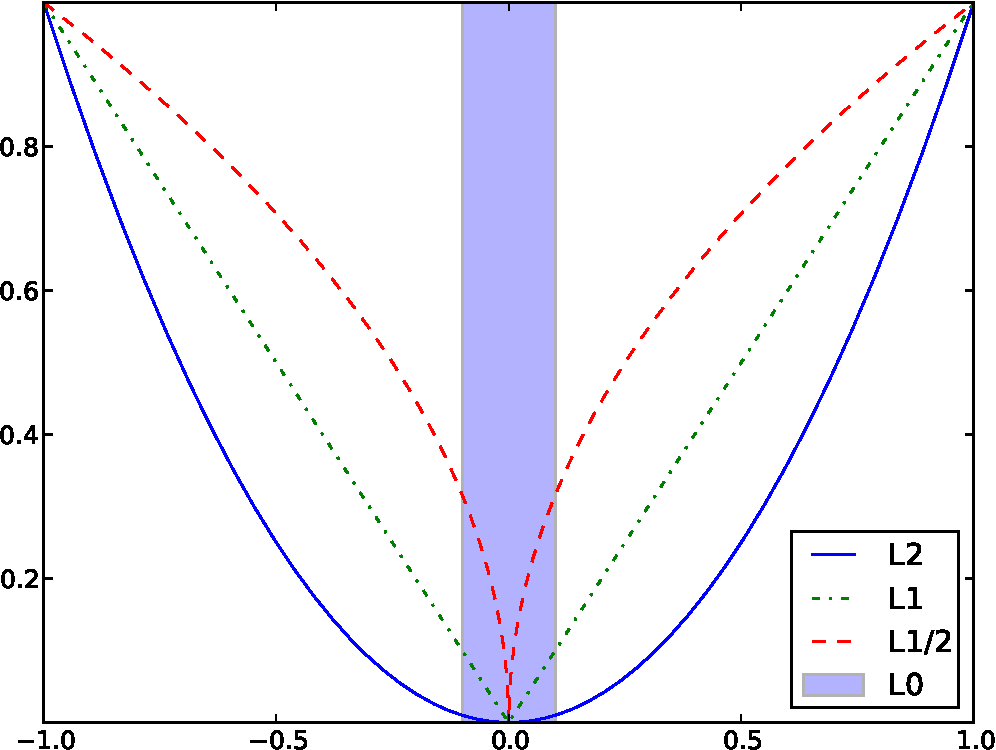
\includegraphics[width=.85\columnwidth]{measures}
\end{center}
\caption{Effect of different measures on one-dimensional data.
\label{fig:measures}}
\end{figure}

\begin{figure}[t]
\begin{center}
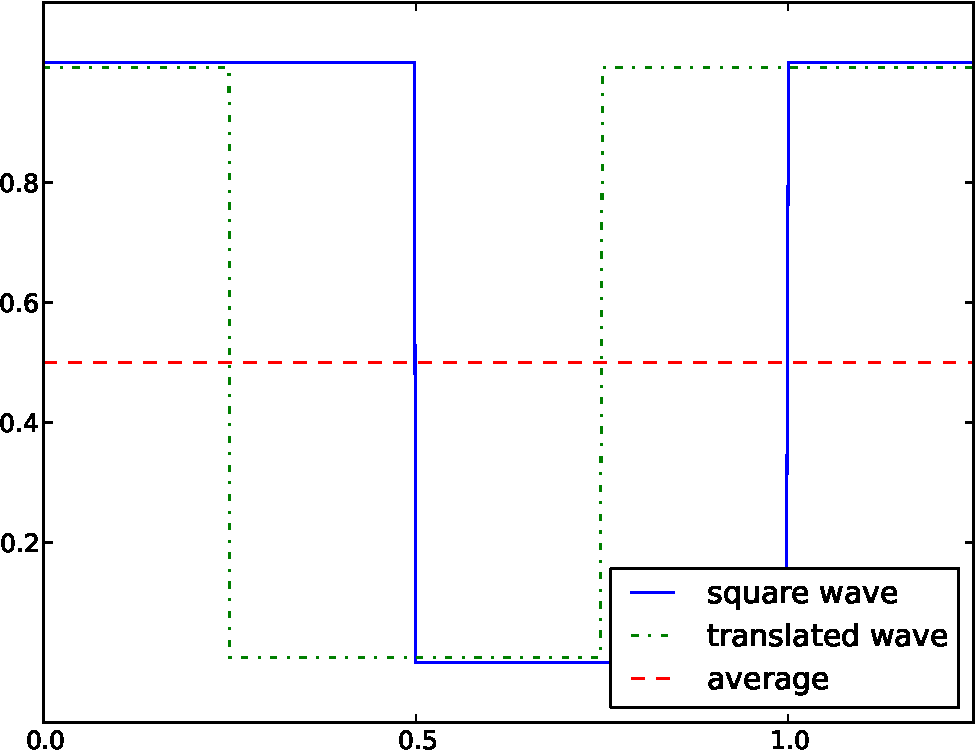
\includegraphics[width=.8\columnwidth]{square}
\end{center}
\caption{Reconstruction error between a square wave and two approximation,
a square wave translated by a quarter of the period, and the average
function. Average error between original and translated wave is always $0.5$
for any Mahalanobis measure $d_p$ on $[0,1]$. 
For the average function, the errors are
$0.25$, $0.5$ and $0.71$ for $d_2$, $d_1$ and $d_{1/2}$ respectively.
\label{fig:square}}
\end{figure}

\section{EXPERIMENTS}
\label{sec:exp}
We present results from different algorithms for imputing masked
beats.  Features are beat-aligned chromas and the dataset is made of
$5000$ songs from the Cowbell dataset
\cite{Bertin-Mahieux2010a}. Songs has to be of length at least $100$
beats.  The masked part is chosen at random, excluding the first and
last $30$ beats.

\subsection{ALGORITHMS}
\label{ssec:algo}
As multi-beat imputation has not been studied before, we report
results on a variety of benchmark algorithms. We realize that such
methods have a low probability of success at solving the task, but
their relative performance is of interest.  Simple methods include
\textbf{random} where each chroma bin is drawn from a uniform $[0,1)$
distribution (Figure \ref{fig:avgnnrand}, $5$th row).  One can also
pick a beat at random from the song, or take the average of all
visible beats. Taking \textbf{average} of the beats within a certain
range of the missing patch (Figure \ref{fig:avgnnrand}, $3$rd row)
create a smooth reconstruction, but still solves the case of
sustained notes.

Our first trained model is linear interpolation (called \textbf{linear transform}
in the text) where we use $N$ previous beats to predict the next one.
As it explicitely learns to minimize Euclidean distance on the visible data,
this methods performs very well under certain metrics (See Figure \ref{fig:basic}).

Nearest neighbor ($\mathbf{1}$\textbf{NN}) is an appropriate tehcnique to take advantage
of the repetitions within a song. By looking at the nearby beats of the missing data,
we can impute a reconstruction by spotting a similar neighborhood. Note that instead
of using the visible part of the song, one can use a \textbf{codebook} made of other songs.
$k$NN with $k>1$ is ongoing research.

We experimented with algorithms with greater representational power, e.g. \textbf{HMM} and
shift invariant probabilistic latent component analysis (\textbf{SIPLCA}) \cite{Smaragdis2009,Weiss2010}.
ADD SOME DETAILS, DIAGONAL/SEQUENCE STATE TRANSITION MATRIX FOR THE HMM, 
RANK AND WIN SIZE FOR SIPLCA.
Due to lack of space and the numerous parameters to tune, we present results without
much details. We refer the reader to our code and mention that this is part of our
ongoing research.


\subsection{RESULTS}
\label{ssec:results}
It is impossible results for every algorithm, measure and number of masked columns.
We selected the most meaningful ones; the reader is referred to our 
website\footnote{Code available at: \url{http://www.columbia.edu/~tb2332/something}}
for data and code to reproduce the results.

Figure \ref{fig:2dscore} shows the performance of $3$ methods for different numbers
of missing beats. We report Euclidean distance and D-ENT. One can see the result
of contradicting measures. Nearest neighbor method ($k=1$) creates a reconstruction
with an entropy similar to the original for all mask sizes. It is a direct consequence
of the fact that entropy is approximately constant throughout a song. The linear
transform learns to minimize the Euclidean distance and does it successfully. But as it
can be seen from its entropy measure and Figure \ref{fig:basic} $3$rd row, it is
done by a large amount of smoothing. The average reconstruction has the same entropy
results than the linear transform, but due to less smoothing (or a less intelligent
one), it does not do as well with the euclidean distance.

\begin{figure}[t]
\begin{center}
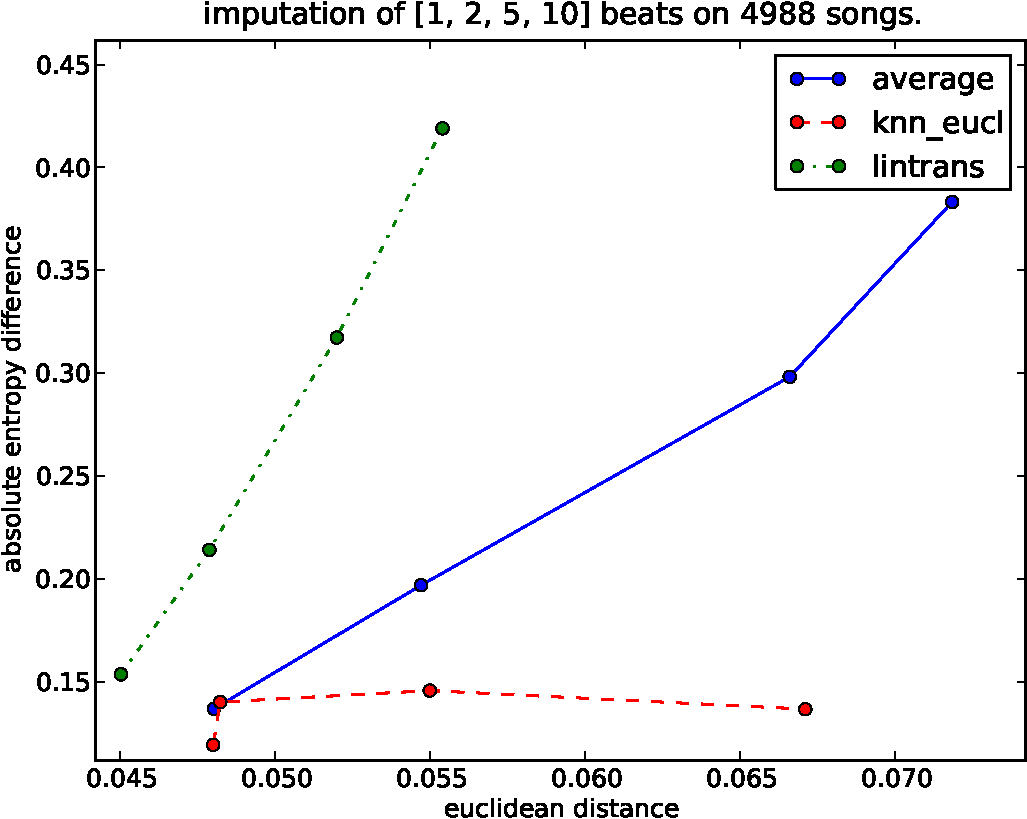
\includegraphics[width=.9\columnwidth]{recon_score_in_2d_5k}
\end{center}
\caption{Reconstruction error for $3$ methods and different
number of masked beats. Errors are D-ENT and Euclidean
distance. In all cases, the larger the number of masked beats,
the higher the Euclidean distance. Lower left is better.
\label{fig:2dscore}}
\end{figure}

In Subsection \ref{ssec:measures} we mentioned many different measures.
We also showed how they could favor different kinds of reconstruction
(with heavy smoothing or not, for instance). To make some sense of
these, we investigate over large set of experiments which measures tend
to agree with each other. We use Pearson's 
correlation\footnote{
$\rho_{X,Y}=\mathrm{corr}(X,Y)={\mathrm{cov}(X,Y) \over \sigma_X \sigma_Y} ={E[(X-\mu_X)(Y-\mu_Y)] \over \sigma_X\sigma_Y}$
} $\rho_{X,Y}$. We have $-1 \leq \rho_{X,Y} \leq 1$, an absolute
value close to $1$ meaning high correlation.
$\rho_{X,Y}$ is computed for many error measures and results are presented in
Table \ref{tab:corrs}. It appears that measures tend to form two groups.
The ``Euclidean-like'' measures favor smoothing to minimize divergence on
average. The ``entropy-like'' measures look at the texture of the reconstruction
compared to the original (ONLY D-ENT IN THAT CATEGORY?????).

\begin{table}[t]
\begin{small}
\begin{center}
\begin{tabular}{|l|c|c|c|c|c|c|} \hline
 & eucl. & cos & KL & D-ENT & $d_{1/2}$ & Jensen \\ \hline
eucl. & $1$ & $0.88$ & $0.77$ & $0.12$ & $0.90$ & $0.84$\\
cos &  & $1$ & $0.91$ & $0.20$ & $0.76$ & $0.97$ \\
KL &  &  & $1$ & $0.17$ & $0.64$ & $0.95$ \\
D-ENT &  & $$ & $$ & $1$ & $0.27$ & $0.20$ \\
$d_{1/2}$ & & & & & $1$ & $0.71$ \\ 
Jensen & & & & & & $1$ \\ 
Leven & $0.59$ & $0.46$ & $0.35$ &$0.41$ & $0.81$ & $0.40$ \\
Thresh. & $0.68$& $0.56$ & $0.46$ & $0.35$ & $0.90$ & $0.51$ \\ \hline

\end{tabular}
\caption{Pearson correlation between measures. Based on all results
from random, average, $1$NN and linear transform on $5000$K songs
with $1$ and $10$ missing beats. $1$ or $-1$ means high
correlation, $0$ means none.
Results form a symmetric matrix, we only show the upper triangle.
\label{tab:corrs}}
\end{center}
\end{small}
\end{table}

We know report results of a $15$ beat imputation on $5000$ songs in
Table \ref{tab:res}. The linear transform is a clear winner based
on Euclidean distance. As before, nearest neighbor's strength
is to preserve the texture of the original patch as can be seen
from his D-ENT score. We can not report all results, but they
are no serious surprises with other measures 
as can be expected from Table \ref{tab:corrs}.

It is a disappointment that powerful methods such as SIPLCA
and HMM did not perform better in our experiments. It
probably only means that more research is needed. HMM should
be extended to model more than one beat at a time. For SIPLCA,
the activation matrix (that tells when each patch is used in time)
should be better constrained via priors for instance.

\begin{table}[t]
\begin{small}
\begin{center}
\begin{tabular}{|l||c|c|c|} \hline
method & Euclidean & KL & D-ENT \\ \hline
random & $0.168$ & $0.461$ & $0.252$ \\
average & $0.079$ & $0.249$ & $0.430$ \\ \hline
1NN & $0.072$ & $0.237$ & $\mathbf{0.123}$ \\
codebook & & & \\ \hline
lin. trans. & $\mathbf{0.056}$ & $0.183$ & $0.479$ \\
SIPLCA & & & \\
HMM & & & \\ \hline
\end{tabular}
\caption{Results on $15$ missing beats by different methods
on $5000$ songs and measured using Euclidean distance and
D-ENT.
\label{tab:res}}
\end{center}
\end{small}
\end{table}

Below are specific examples of original / reconstruction pairs.

\begin{figure}[t]
\begin{center}
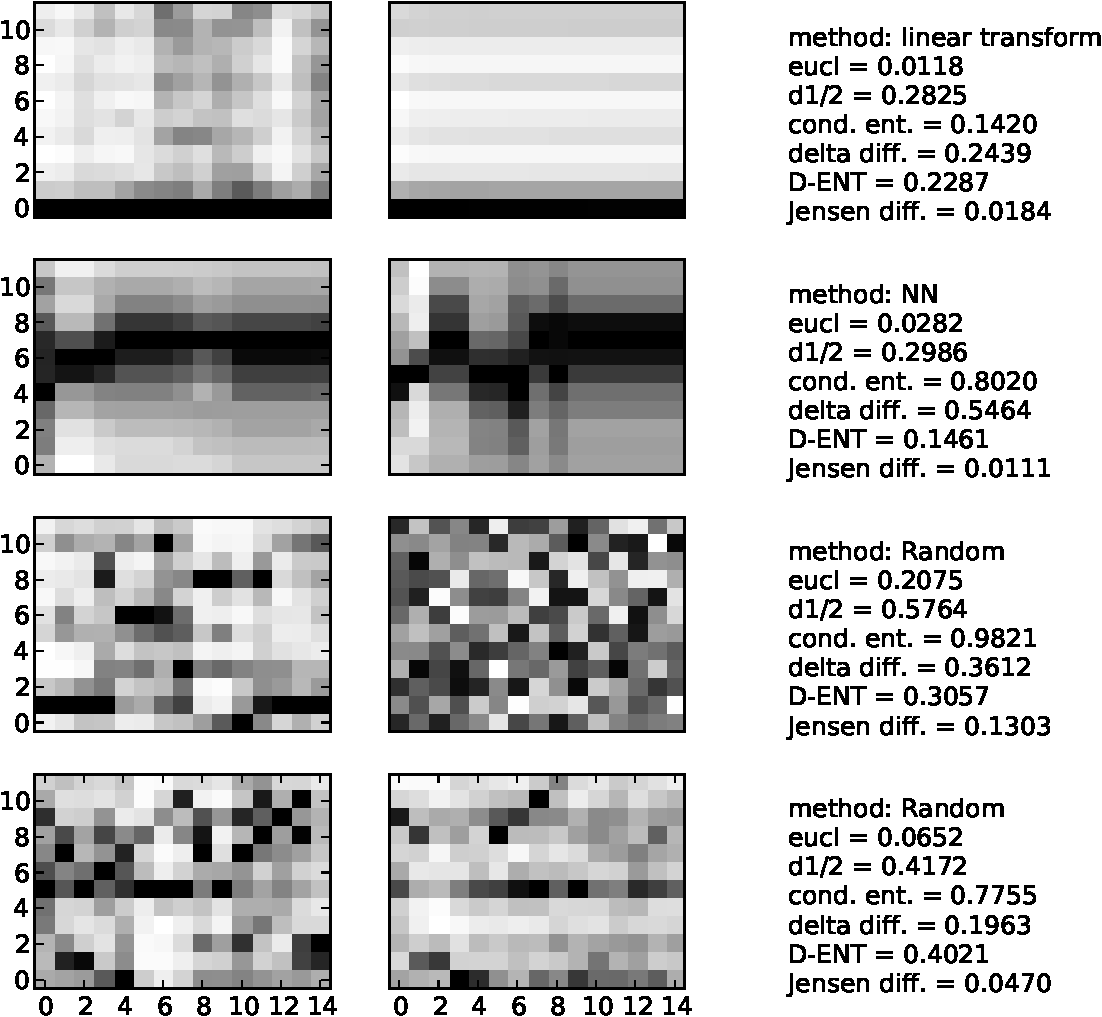
\includegraphics[width=.9\columnwidth]{original_recons}
\end{center}
\caption{Selected pairs of original patches ($1$st column)
and their reconstructions ($2$nd column). 
Method used and some error measures
reported on the right.
\label{fig:origrecon}}
\end{figure}



\iffalse
\begin{table}[t]
\begin{small}
\begin{center}
\begin{tabular}{l|c|c|c|c|c|}
\# beats  & 1 & 2 & 5 & 10 & 15 \\ \hline \hline
random & $0.166$ & $0.166$ & $0.167$ & $0.167$ & $0.168$  \\
rand. song & $0.115$ & $0.114$ & $0.114$ & $0.115$ & $0.115$  \\
average all & $0.057$ & $0.057$ & $0.057$ & $0.057$ & $0.058$ \\
average & $0.047$ & $0.053$ & $0.062$ & $0.065$ & $0.069$ \\ \hline
knn eucl & $0.048$ & $0.049$ & $0.055$ & $0.064$ &  $0.070$ \\
knn kl & $0.049$ & $0.050$ & $0.056$ & $0.066$ &  $0.071$ \\
lin. trans. & $\mathbf{0.044}$ & $\mathbf{0.047}$ & $\mathbf{0.051}$ & $\mathbf{0.053}$ & $\mathbf{0.055}$ \\
codebook & & & & &  \\
SIPLCA & & & & &  \\ \hline
\end{tabular}
\caption{Results based on euclidean distance on $43K$ songs.
Song has to be at least $70$ beats long. 
For ``average'', window is $2$ beats each side of the masked patch.
For ``knn eucl'' and ``knn kl'', window is $10$ beats each side of the masked patch.
For ``lin. trans.'', window is the $2$ previous beats.}
\label{tab:reseucl}
\end{center}
\end{small}
\end{table}

\begin{table}[t]
\begin{small}
\begin{center}
\begin{tabular}{l|c|c|c|c|c|}
\# beats & 1 & 2 & 5 & 10 & 15 \\ \hline \hline
random & $0.428$ & $0.450$ & $0.461$ & $0.461$ & $0.462$  \\
rand. song & $0.334$ & $0.351$ & $0.371$ & $0.377$ & $0.380$  \\
average all & $0.164$ & $0.175$ & $0.183$ & $0.187$ & $0.189$ \\ 
average & $0.121$ & $0.154$ & $0.194$ & $0.212$ &  $0.223$ \\ \hline
knn eucl & $\mathbf{0.116}$ & $0.136$ & $0.169$ & $0.212$ & $0.233$ \\
knn kl & $\mathbf{0.116}$ & $\mathbf{0.135}$ & $\mathbf{0.167}$ & $0.209$ & $0.229$ \\
lin. trans. & $0.141$ & $0.157$ & $0.170$ & $\mathbf{0.180}$ & $\mathbf{0.184}$ \\
codebook & & & & &  \\
SIPLCA & & & & &  \\ \hline
\end{tabular}
\caption{Results based on symmetric KL divergence on $43K$ songs.
See Table \ref{tab:reseucl} for the exact parameters used.}
\label{tab:reskl}
\end{center}
\end{small}
\end{table}
\fi

\section{CONCLUSION AND FUTURE WORK}
\label{sec:conclusion}
As mentioned, modifications of HMM and SIPLCA are ongoing
research. There is great hope that algorithms pretrained
on large additional data (another set of songs) will break
the curse of boring smoothed patterns.
A unified set of measures should also be selected
by the community. Our code and test data is available to 
reproduce and improve these results.


%\section{ACKNOWLEDGEMENTS}
%NSERC PG grant for Thierry, something for Ron, NSF from Dan.


% References should be produced using the bibtex program from suitable
% BiBTeX files (here: strings, refs, manuals). The IEEEbib.bst bibliography
% style file from IEEE produces unsorted bibliography list.
% -------------------------------------------------------------------------
\bibliographystyle{IEEEbib}
\bibliography{tbm_bib}

\end{document}
